%!TEX root = ../main.tex
\section{System Implementation and Testing}
This section will describe how the system was implemented and tested on both a test setup and the real go-kart setup. 

\subsection{Test Setup}
In order to test subparts of the complete system a test setup was introduced.
It consists of a permanent magnet motor of the type PM5113 with a RMB28MD encoder module mounted with a small distance to the end of the shaft.
The setup furthermore consists of a 74HCT14 level shift interface board and a ??\todo{Thomas: Questionmark?} dual H-bridge and can be seen in figure \ref{fig:small_motor_setup}.
The setup was made and soldered by the supervisors of the project.
The full setup with H-bridge can be used to test the functionality of the Embedded System.
The motor and encoder can be used to test the full system.

\begin{figure}[!h]
	\centering
	\includegraphics[width=0.8\linewidth]{graphics/small_motor_setup}
	\caption[Block diagram of test setup.]{Block diagram of test setup with PM5113 motor.}
	\label{fig:small_motor_setup}
\end{figure}

\todo[inline]{The figure is wrong!! signal should go two times in the level shifter - Mikkel}

\subsection{PWM generating}
To test whether or not the Clarke Park transformation and the PWM generating on the Zybo board was working correctly a test was conducted.
The test setup, described in the previous section, was used.
The three legs of the H-bridge was connected to the control pins for the upper MOSFETS for phase a, b and c.
A constant value for q was chosen and d was set to zero. 
The angle of the rotor was measured and used to do the Clarke Park transformation. 
No current measurements were done, meaning that the only feedback was the angle.
Each of the signals from the output pins of the Zybo board were, in addition to the H-bridge, connected to an electric lowpass filter consisting of a 10 \si{\kilo\ohm} resistor and a 22 \si{\nano\farad} capacitor. 
The voltage across the capacatior was measured by an oscilloscope as the power supply for the H-bridge was turned on.
The measured phase voltages can be seen in figure \ref{fig:small_motor_phases}.
It can be seen that the three phase voltages are created correctly by the Zybo board.
It can also be seen that the rotor is accelerated within a fraction of an electrical revolution, which is expected as there is no torque load. 

\todo[inline]{I am pretty sure this is before third harmonic injection was working! - Mikkel}
\begin{figure}[!h]
	\centering
	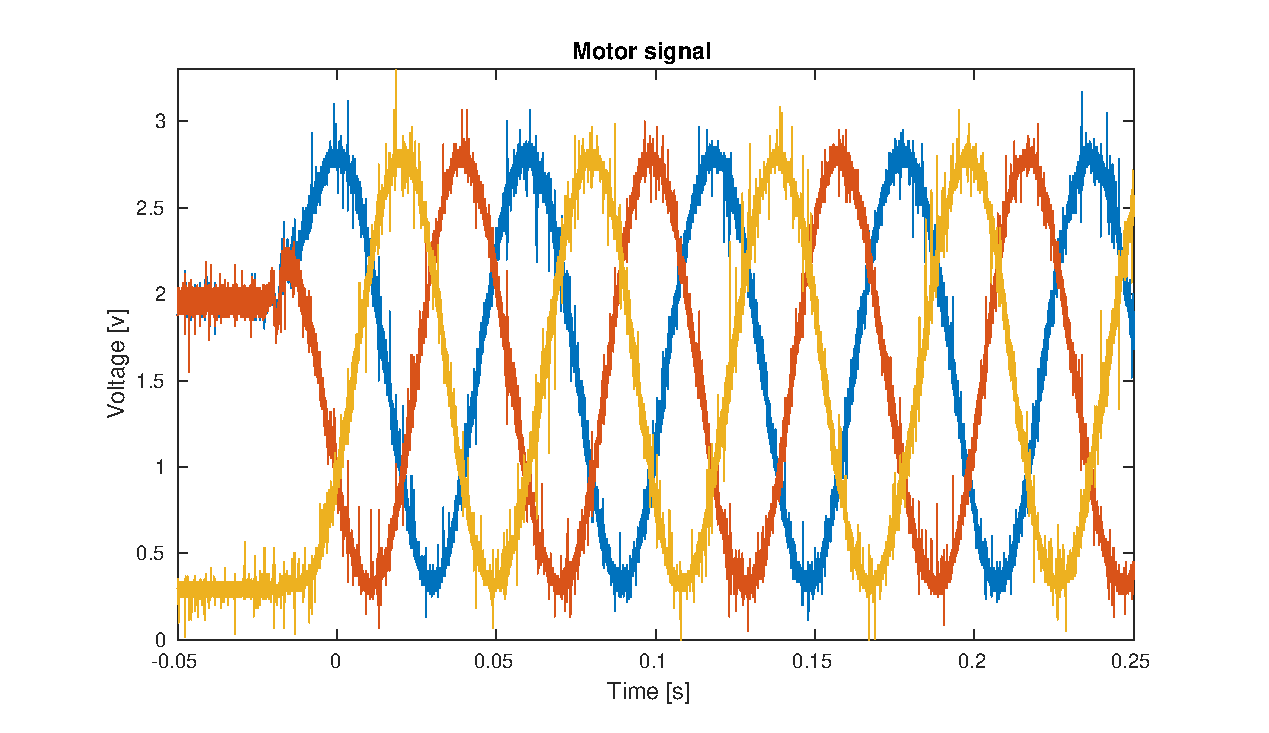
\includegraphics[width=1\linewidth]{graphics/small_motor_phases}
	\caption[Phase voltages.]{Phase voltages measured through a lowpass filter.}
	\label{fig:small_motor_phases}
\end{figure}

\subsection{Analog, Digital and Driver Boards}
\todo[inline]{Thomas: I think it would be advisable to have someone else read through this to ensure that it is not too emotional... I dislike making excuses..}
Various issues were encountered while creating prototypes of especially the analog and digital boards.
Several iterations were etched before a satisfactory result was obtained.
Due to delivery issues, the components were not available until very late in the process and there was not sufficient time remaining to fully debug the boards.
The driver board was made to function as was intended and is used in section \todo[inline]{Thomas: section that describes testing of the power board.}.
As mentioned in previous sections, the strategy used for OCP changed throughout the testing phase.
It became apparent that it was infeasible to spend the time necessary to have the analog board functioning in time for the deadline.
In the meantime the OCP of the DRV8301 was understood, allowing to use this feature instead.\\

As shown in section \ref{sec:electricsimulation}, the general behaviour of the OCP circuit is working as intended.
The errors found on the analog and digital boards are mostly related to layout and unintentional short circuits.
For this reason it is the conviction of the group that one or two revisions of the boards would be necessary to fully debug them.
